
\section{Introduction}

The NIME community (New Interfaces for Musical Expression) is rich, diverse, and ever expanding. New technologies are continually developed, allowing creatives to interact with machines to create sonic artifacts and experiences that would not have been possible otherwise \citep{wanderley_gestural_2001}. 

This paper aims to explore the ways in which the expressive capacity of the guitar can be extended by employing new techniques and technologies to this familiar and well-loved instrument.

This will be achieved by the development of an experimental prototype MIDI controller which will incorporate new MPE (MIDI Polyphonic Expression) techniques which allows users to create more expressive performances by allowing pitch and volume manipulations on a per-note basis. This is of course supported on existing traditional guitars, but is not found on contemporary guitar-like MIDI controllers such as the Yamaha EZ-EG \citep{yamaha_yamaha_2003}. Something which has surprisingly not been supported as standard in MIDI since its inception in 1982, and has recently seen an uptick in adoption and implementation.

The prototype achieves its goals by implementing multi-touch capacitive sensors (Bela Trill Bar) across the frets of the guitar, which afford data on touch position and touch size, which can be combined to determine appropriate note-on and off events, to emulate the playing of a guitar. However, this can also be used to create expressive aftertouch and pitch bend data, which is central to the thesis of this study. 

This paper follows three themes which can be summarised by the following questions:
\begin{enumerate}
    \item What are interesting ways to extend the expressive vocabulary of the guitar as a MIDI controller?
    \item How can we create a digital MIDI instrument that guitarists will enjoy using and be conducive to creative flow?
\end{enumerate}

Creative flow is defined as ``\textit{the mental state in which a person performing some activity is fully immersed in a feeling of energized focus}" \citep{csikszentmihalyi_flow_1990}. \cite{macdonald_creativity_2006} highlight how important flow is to productive and creative musical output. Enabling creatives with digital instruments that can interface with modern tools such as Digital Audio Workstations and modern synthesizers with an interface that is conducive to a state of creative flow, is the key motivation of this paper. \textit{Creatives}, in this context, is defined as any person using (digital music technology) to create novel creative output, such as songs or audio artefacts. 

Some studies indicate that there is a feeling among creatives that interaction with digital audio units or MIDI instruments is not conducive to creative flow \citep{martelloni_percussive_2020}. This perception is a key challenge to this paper. The author proposes that this is not an intrinsic property of digital instruments, but instead is product of the relative novelty of these digital technologies, whose designs have not been iterated and smoothed-out over generations of musicians. The traditional guitar, over it's near half a millennium of existence \citep{tyler_renaissance_1975}, has had the chance to have its design iterated and improved by great numbers of people. The MIDI guitar has had mere decades, so it is no surprise that (currently) the design does not compare to its traditional counterpart. This study attempts to take one more step in the iterative process of the collective goal of designing the digital MIDI guitar. 






























% Since the development of the electric guitar and amplifier in <DATE> by <PERSON> \cite{SOMETHING}, the guitar has had a rich history of technological augmentation. Guitarists have benefited from the creative technological advances, for example, the compact electronic design in pedals \cite{SOMETHING}, and more recently the development of VST and other DAW plug-in technologies and effects to further their creative possibilities \cite{SOMETHING}.

% This paper will focus on the digital augmentation of the guitar, as described by Marcelo Wanderley \cite{wanderley_gestural_2001}, as a \textit{instrument-like controller} (ILC); for example the Yamaha EZ-AG as seen in Figure \ref{fig:yamaha_wx7}. ILCs are a subset of NIME which are inspired by existing traditional instruments, but whose sound is not necessarily related to the sound of the original instrument.

% \begin{figure}[h]
%     \centering
%     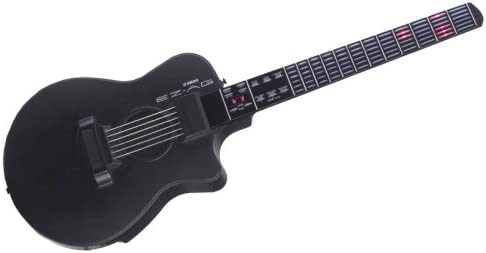
\includegraphics[scale=0.4]{Images/ezag.jpg}
%     \caption{The Yamaha EZ-AG is an \textit{instrument-like controller}.}
%     \label{fig:yamaha_wx7}
% \end{figure}

% There are a number of key motivating factors for this research, which arise from the constraints of traditional guitars, music information retrieval (MIR) based augmentation, and current guitar-based ILC up to this point.  

% The key motivations and themes of this work are outlined below.

% % =================================================
% \vspace{15pt}

% \begin{enumerate}
%     \item \textbf{Limitations of MIR based approaches}. Explain why MIDI pick ups aren't perfect, and why they may block creative flow, which is key to everything. How might MIR approaches work? Mention the traditional polyphonic approach or fret detection/resistance measurement. 
%     \item \textbf{Expanding the gestural palette for guitar-based ILC}. What are the drawbacks of ILDs like the Yamaha EZ-EG, and Starr Labs Explain why it could empower new kinds of expression for guitarists, which would be awesome. We want to support the tapping-style techniques which are demonstrated by MIDI guitar practitioners such as Rob Swire \cite{log_starr_2011} and Fabrizio Chiruzzi \cite{fabrizio_chiruzzi_channel_what_2010}.
%     \item \textbf{Guitar based MIDI control for composition professionals}. Explain why it would be useful to enable composers and producers to input musical data in a way which is most conducive to their muscle memory and creative flow. 
%     \item \textbf{Designing for true ambidextrous use}. Why is it important that products are able to support both right and left-handed users equally, and still be an appealing product to both, make sure you mention Norman \cite{norman_design_2013}.
%     \item \textbf{Inclusive design for limb-different users}. There has been generally very little support for guitarists with disabilities affecting the arms and upper body \cite{SOMETHING}, though, there has been great progress made by individual practitioners to develop techniques and technologies that support their creative vision. 
% \end{enumerate}

